\documentclass[review]{elsarticle}
\usepackage{graphicx}
\usepackage{amsmath}
\usepackage{enumerate}
\usepackage{multirow}
\usepackage{epstopdf}
\usepackage{array}
\usepackage{CJK}
\usepackage{float}
\usepackage{subfigure}
\usepackage{algorithm}
\usepackage{algorithmicx}
\newcommand{\algorithmicbreak}{\textbf{break}}
\newcommand{\BREAK}{\State \algorithmicbreak}
\usepackage{algpseudocode}
\newtheorem{problem}{\textbf{Problem}}
\usepackage{lineno,hyperref}
\modulolinenumbers[5]

\journal{Journal of \LaTeX\ Templates}

%%%%%%%%%%%%%%%%%%%%%%%
%% Elsevier bibliography styles
%%%%%%%%%%%%%%%%%%%%%%%
%% To change the style, put a % in front of the second line of the current style and
%% remove the % from the second line of the style you would like to use.
%%%%%%%%%%%%%%%%%%%%%%%

%% Numbered
%\bibliographystyle{model1-num-names}

%% Numbered without titles
%\bibliographystyle{model1a-num-names}

%% Harvard
%\bibliographystyle{model2-names.bst}\biboptions{authoryear}

%% Vancouver numbered
%\usepackage{numcompress}\bibliographystyle{model3-num-names}

%% Vancouver name/year
%\usepackage{numcompress}\bibliographystyle{model4-names}\biboptions{authoryear}

%% APA style
%\bibliographystyle{model5-names}\biboptions{authoryear}

%% AMA style
%\usepackage{numcompress}\bibliographystyle{model6-num-names}

%% `Elsevier LaTeX' style
\bibliographystyle{elsarticle-num}
%%%%%%%%%%%%%%%%%%%%%%%

\begin{document}

\begin{frontmatter}

\title{Exploiting Publication Contents and Collaboration Networks for Collaborator Recommendation}
%\tnotetext[mytitlenote]{Fully documented templates are available in the elsarticle package on \href{http://www.ctan.org/tex-archive/macros/latex/contrib/elsarticle}{CTAN}.}

%% Group authors per affiliation:
\author{Elsevier\fnref{myfootnote}}
\address{Radarweg 29, Amsterdam}
\fntext[myfootnote]{Since 1880.}

%% or include affiliations in footnotes:
\author[mymainaddress,mysecondaryaddress]{Elsevier Inc}
\ead[url]{www.elsevier.com}

\author[mysecondaryaddress]{Global Customer Service\corref{mycorrespondingauthor}}
\cortext[mycorrespondingauthor]{Corresponding author}
\ead{support@elsevier.com}

\address[mymainaddress]{1600 John F Kennedy Boulevard, Philadelphia}
\address[mysecondaryaddress]{360 Park Avenue South, New York}

\begin{abstract}
In academia, studies have shown that researchers are usually prolific through effective collaboration with other researchers in the same field. However, due to the expansion of academic research in diverse domains, the problem of finding the most relevant and potential collaborators (MPCs) from a large volume of big scholarly data has become cumbersome and time-consuming. In this work, we propose an academic collaborators recommendation model called CCRec. CCRec is an innovative model that combines content-based and social network-based methods. In order to effectively seek the most potential collaborators for researchers, we adopt a topic clustering model as well as a random walk model. Using DBLP data sets, we conduct benchmarking experiments to examine the performance of CCRec. In addition to addressing the topic drift problem, our preliminary experimental results show that CCRec outperforms other state-of-the-art methods in precision, recall and $F1$ score.
\end{abstract}

\begin{keyword}
Collaboration recommendation, publication contents, collaboration networks, topic clustering, random walk.
\end{keyword}

\end{frontmatter}

\linenumbers


% =============================================================================
\section{Introduction}
% =============================================================================
Nowadays, the current scale of the Internet has risen beyond the imagination of people due to its rapid development. The Internet has gradually shown its ability of being the main carrier for sharing information. Consequently, how to obtain useful and effective information has become a complex task as a result of information overload. Therefore, recommender systems and techniques immensely help people by providing easier access to the specific resources they really need.

In academia, cooperation among researchers is of vital necessity. Studies have shown that collaboration is a considerable factor to consider in relation to the productivity of a scholar \cite{lee2005impact}. Therefore, researchers tend to discover the most potential collaborators (MPCs)i.e. some influential scholars who have similar research interests and have never collaborated with before, or reinforce the collaboration with the most valuable collaborators (MVCs)i.e. some influential scholars or colleagues who are active and valuable in adjacent circles and have collaborated in the past. Considering the inherent requirements, a variety of methods relating to collaborators recommendation have been proposed. These methods involve both collaboration and non-collaboration among researchers.

In this context, previous studies have exploited three main aspects for academic collaboration recommendation, content-based, social network-based and hybrid recommendation. Some traditional content-based methods extract researchers academic features through interests tags, user profiles, publications etc, then make collaborators recommendation by computing interest similarities \cite{lopes2010collaboration,gollapalli2012similar,kim2010collaborative}. However, in general, a researcher shows biasness in various academic domains. Such behaviors usually reveal academic features of researchers in different domains. Thus, it is imperative to consider academic domains when recommending collaborators. Our previous work proposed a social network-based model called ACRec \cite{li2014acrec}, which solved the problem of recommending MVCs. ACRec makes it easier for scientists to collaborate with colleagues in their social networks. However, many scientists also initiate collaborations outside of their social networks. It is burdensome and fraught with risk of initiating collaboration with socially unconnected researchers. In addition, considering the less value of recommending already known collaborators, unconnected researchers are more deserve to be recommended as MPCs. What's more, some excellent hybrid models have been introduced in recent years \cite{lee2011recommending,chen2011collabseer,cohen2013recommending}, which have paved the way for many good references.

In this paper, we propose a novel hybrid model exploiting Publication Contents and Collaboration Networks for Collaborators Recommendation (CCRec). Utilizing a topic clustering model \cite{pan2010research} \cite{pham2011clustering} and a random walk model, CCRec integrates the features of publications contents and collaboration networks. We extract the subject terms from all researchers' publications and cluster these terms into several topics, then distribute researchers to corresponding domains. To represent the feature vectors of each researcher, we run the random walk with restart model (RWR) on each domain, which has been proved to be competent for calculating the rank score of nodes in social networks. After that, the MPCs recommendation is provided by computing the similarities of researchers' feature vectors.

In summary, we make the following contributions in this paper. 1) To compute the most potential collaborators recommendation, we develop a model CCRec, which combines the content-based and social network-based methods. By adopting this procedure, our approach is more favourable in terms of achieving remarkable personalized collaborators recommendation. 2) To reveal researchers' academic features in different domains, we present the feature vectors by utilizing a topic clustering model and a random walk model. 3) Finally, conduct extensive experiments on a subset of DBLP data set to evaluate the performance of CCRec in various scenarios in comparison to our previous ACRec model and the normal common neighbors-based model (CNRec). Promising results are presented and analyzed.

The remainder of the paper is structured as follows. Section 2 briefly presents the related work. We discuss the details of our recommendation model in section 3, which highlights the structure of the model. In section 4, we conduct a series of experiments and analyze the results. Finally, section 5 concludes the paper.

% =============================================================================
\section{RELATED WORK}
% =============================================================================
Collaboration plays an important role in academic research. A large body of work relating to academia focuses on two key issues, reinforcing and discovering collaborators, which are respectively defined as MVCs recommendation and MPCs recommendation in this work. Lopes et al. \cite{lopes2010collaboration} worked on identifying new partners to execute joint research and enhancing the cooperation of current partners for researchers. Chen et al. \cite{chen2009make} proposed that the purpose of friends recommendation is "Make new friends, but keep the old". Research on enterprise social networking \cite{dimicco2008motivations} shows that users in a corporate context are interested in discovering valuable contacts not yet known to them, or connecting to weak ties, in addition to staying in touch with their close colleagues. Our previous work \cite{li2014acrec} focuses on recommending MVCs for researchers and enhancing the cooperation with colleagues in their academic social networks. In this work, CCRec has an aptitude for discovering new collaborators with high similarity (i.e. MPCs recommendation).

In general, collaborators recommender systems are studied in three different perspectives according to the following methodologies used to perform recommendation: \emph{content-based}, \emph{social network-based} and \emph{hybrid approach}. The related work presented below correlate with these types of models.

\emph{content-based}, which recommends items classified according to user profiles and early choices considering semantic issues. Das G. et al. \cite{gollapalli2012similar} proposed models for computing the similarity between researchers based on expertise profiles extracted from their publications and academic homepages. Lopes et al. \cite{lopes2010collaboration} considered researchers' publications area and the vector space model to make collaboration recommendation. Kim et al. \cite{kim2010collaborative} proposed a collaborative filtering method to provide an enhanced recommendation quality derived from user-created tags. However, researchers often behave differently across multiple domains of interests, which might introduce topic drift problems in general recommendation systems \cite{tang2012cross}.

\emph{social network-based}, which recommends items considering the structure of social networks or some social factors. Ma et al. \cite{ma2011recommender} analysed how social network information can benefit recommender systems and proposed a method of improving the performance of recommender systems by incorporating social network information. T. Huynh et al. \cite{huynh2013trend} proposed a method based on a combination of probability theory and graph theory for modeling and analysing co-author networks. They explored similar vertices of potential candidates for collaboration recommendation. Their main contribution involves taking the trend information into considering similarity of vertices. Many other approaches have been presented to formalize academic collaboration recommendation as a link prediction problem \cite{chen2012discovering} \cite{sun2011co} in social networks. Some of these approaches have been applied to large social networks and results show good performance. Lichtenwalter et al. \cite{lichtenwalter2010new} examined some important factors for link prediction and proposed a general framework, in addition to our previous work \cite{li2014acrec}.

\emph{hybrid}, which combines the content-based and social network-based method to integrate their benefits. Lee et al. \cite{lee2011recommending} exploited how well content-based, social network-based and hybrid recommendation algorithms predict coauthor relationship, and results show that a hybrid algorithm combining content and social networks information performs better. Chen et al. \cite{chen2011collabseer} discussed CollabSeer, an open system to recommend potential research collaborators for scholars and scientists, which discovers collaborators based on the structure of coauthor networks and the user's topic of research interests. Cohen et al. \cite{cohen2013recommending} also worked on solving the collaborators recommendation problem, by combining traditional techniques for structural link prediction in social networks with textual relevancy and global importance metrics.

% =============================================================================
\section{DESIGN OF CCRec}
% =============================================================================
Our proposed recommendation scheme for CCRec is inspired by the reality and truth that a researcher usually desires to know other researchers who have similar research interests and strong influence in academia. As mentioned above, researchers often behave differently across multiple domains of interests. Such behaviors usually reveal the academic features of researchers in different domains. Besides, as a social-based model, the RWR model has been proved to be competent for calculating the rank score of nodes in social networks derived from co-authorship \cite{li2014acrec}, researchers' strength of influence in specific domains can be well reflected by RWR. In this work, we first adopt a content-based method to acquire multiple domains of interests. With utilizing a content-based method, we then employ the social network-based method of RWR to measure the researchers' strength of influence in different domains. In the final step of our design, we use the feature vector to evaluate the similarity of researchers and then obtain the recommendation list. The detailed process is described below and the corresponding pseudo-code is illustrated in Algorithm 1. Figure 1 depicts the three main components of CCRec.

%Initially,

%In this work, we proposed a content-based method to acquire multiple domains of interests. Furthermore, we define the SoI (Strength of Influence) to denote the %academic values (Rank Score) of researchers in different domains, which can be regarded as the elements of feature vector of researchers. Finally,we use the %feature vector to evaluate the similarity of researchers and then obtain the recommendation list.
%Topic clustering and researcher partition distribute researchers according to multiple domains.
\begin{figure}
\centering
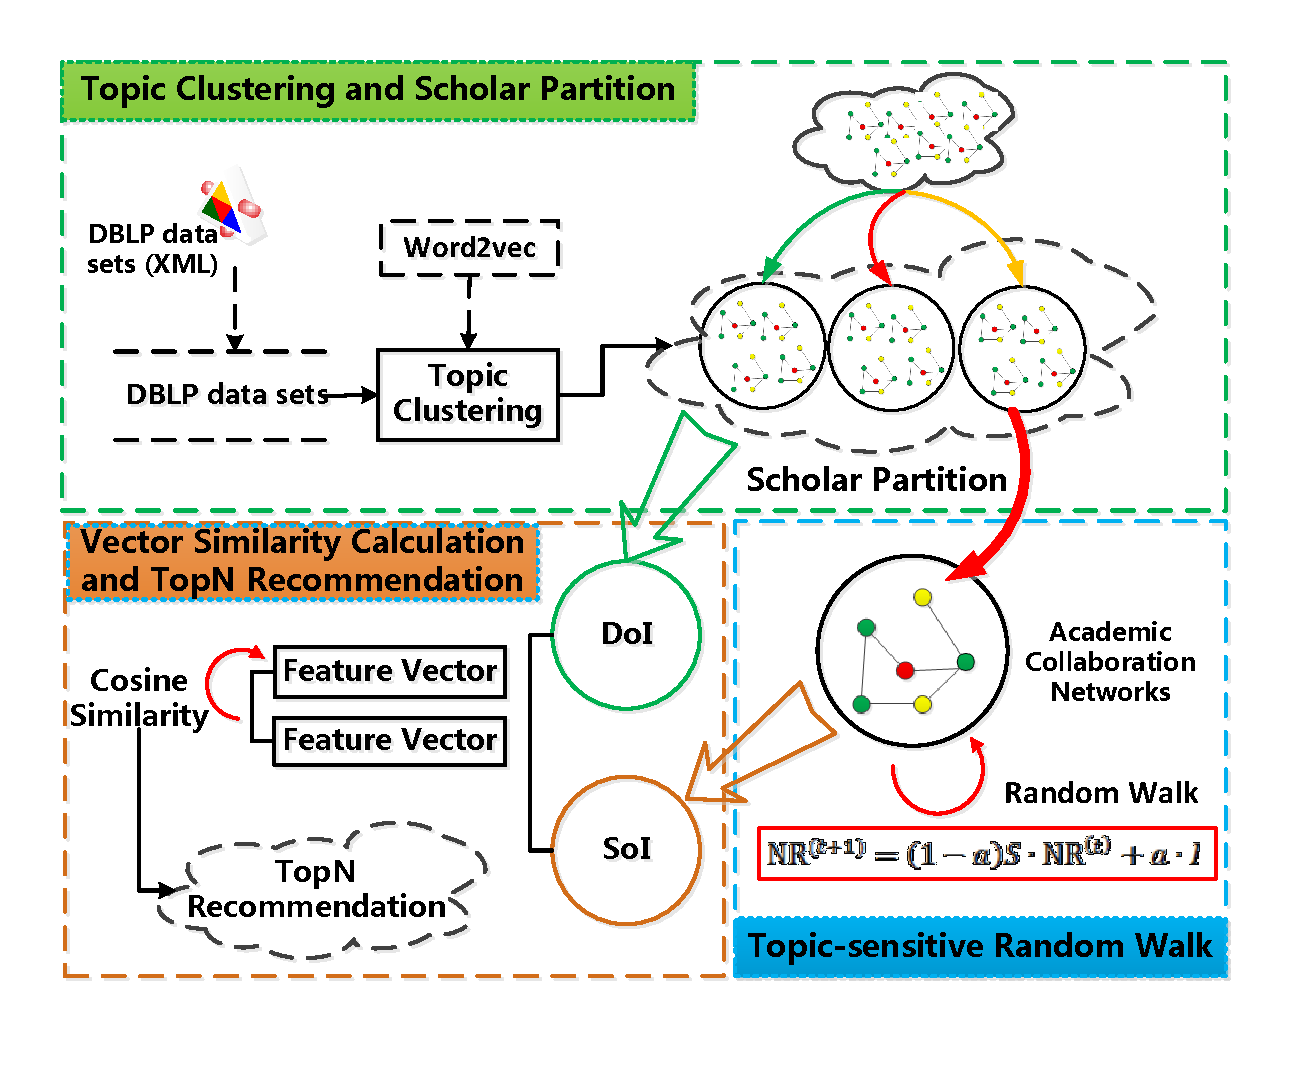
\includegraphics [width=4in]{Fig1.pdf}
\caption{The architecture diagram of CCRec model}
\end{figure}

\subsection{Topic Clustering and Researcher Partition}
% -----------------------------------------------------------------------------
It is a content-based method for topic clustering and researcher partition, which generates various domains and maps all researchers into these domains. In this work, we use a famous tool of Natural Language Processing (NLP) called word2vec, which provides an efficient implementation of the continuous of \emph{bag-of-words} and \emph{skip-gram} architectures for computing vector representations of words. It takes a text corpus as the input and produces the word vectors as the output. The final word vector file can be used as features in many NLP and machine learning applications. The word vectors can be also used for deriving word classes from huge data sets. This is achieved by performing K-means clustering on top of the word vectors. The output is a vocabulary file with words and their corresponding domain IDs. In the case of our CCRec model, the input data is a set of titles from all the papers created by each researcher. The titles are split in many sequential words. In addition, it is necessary to filter out some irrelevant words, e.g. "of", "the", "and", etc. When extracting words from titles, the set of preprocessed words can be used outline the core contents of papers, which are signified as valuable and reliable corpus to denote a variety of academic topics. With this English corpus, word2vec obtains various domains and clusters the words into specific domains.

In addition, CCRec partitions researchers to specific domains through the following methods (i) Extract subject terms from a researcher's publications and (ii) Traverse all the terms and check the word vector. The model tags the researcher for particular domains that contain these subject terms. It should be emphasized that one researcher always belongs to several domains and there are also many researchers in one domain. Fig. 2 illustrates an example. Assuming that CCRec extracts 12 subject terms from the publications titles of researcher $S1$. After topic clustering, we can see that, three of these subject terms are assigned to domain $A$, seven in $B$, and two in $C$. Thus, researcher $S1$ is tagged for domains $A$, $B$ and $C$. Through this method, each domain contains numerous researchers.

\subsection{Feature Vector Calculation}
% -----------------------------------------------------------------------------
As mentioned in section 2, in general, researchers devote themselves to several adjacent domains. But in the case of attention and strength of influence in various domains, there are often some biases. To measure the distribution of researchers' interests, we define the $SoI$ (Strength of Influence) to denote the academic values (Rank Score) of researchers in different domains, which can be regarded as the feature vector elements of researchers. Considering each of the domains, there are numerous researchers with similar research interests. Their co-author relationships can be modeled by a social network. Thus, there are many co-author networks corresponding to different domains. The $SoI$ is measured by RWR model based on the co-author networks. The core equation of the RWR model is shown in equation (1) below:
\begin{equation}
R_{d}^{(t+1)}=\alpha \mathbf{S}R_{d}^{(t)}+(1-\alpha)q
\end{equation}
where $R_{d}$ represents the rank score vector of all researchers in domain $d$, $q$ is the initial vector $R^0$, and $\alpha$ denotes the damping coefficient. RWR is an iterative process. After limited iterations, the vector $R$ will be convergent. In this scenario, $SoI_{s}=R_{d,s}$. That is, the final value of the vector item $R_{d,s}$ is the $SoI$ of researcher $s$.


In addition, with the help of RWR, the $SoI$ in various domains is quantified for each researcher. To measure researchers' academic feature, we define the vector $F$ with $SoI$.

\begin{figure}
\centering
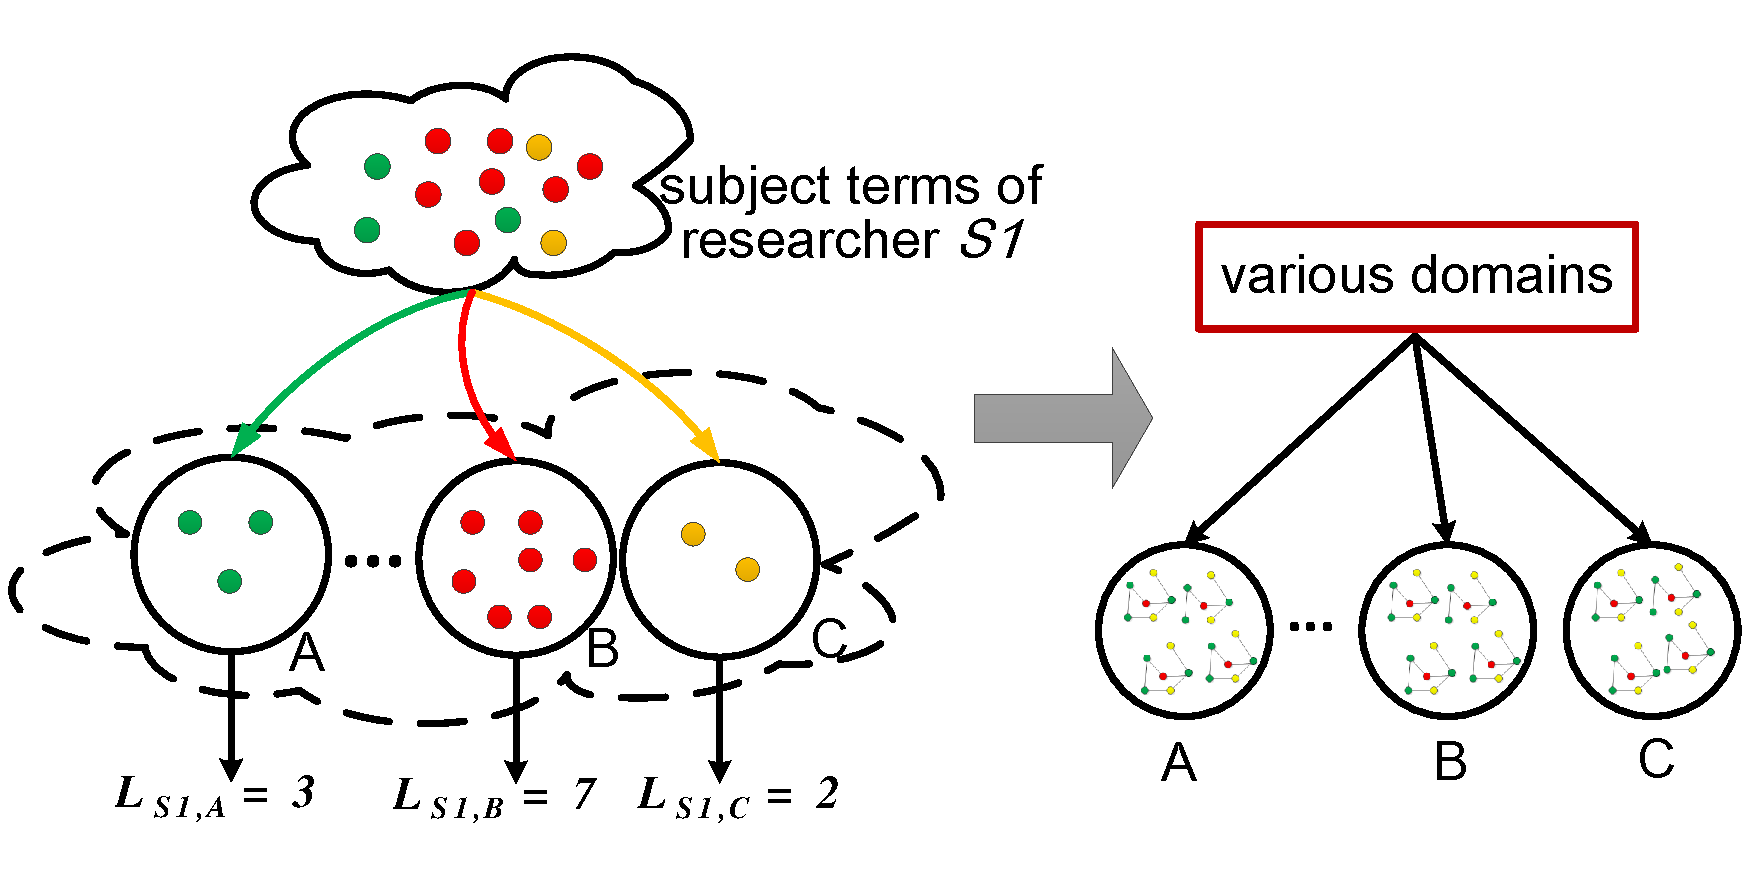
\includegraphics [width=4in]{Fig5.pdf}
\caption{Researcher Partition}
\end{figure}

\subsection{Collaboration Recommendation by Feature Vector Similarity}
% -----------------------------------------------------------------------------
CCRec recommends collaborators for researchers based on their similarities. To measure the academic feature similarities of researchers, we borrow a standard method, \emph{cosine similarity} (CS). CS is employed to define the similarity between two users $s_{1}$ and $s_{2}$ based on their feature vectors $F_{s_{1}}$ and $F_{s_{2}}$.
\begin{equation}
Sim(s_{1},s_{2})=\frac{\sum_{i=1}^{n}(F_{s_{1},i}*F_{s_{2},i})}{\sqrt{\sum_{i=1}^{n}F_{s_{1},i}^2}*\sqrt{\sum_{i=1}^{n}F_{s_{2},i}^2}}
\end{equation}
Finally, we consider that researchers with high similarities have common interests. Therefore, they should be recommended to each other as potential academic collaborators. Hence, CCRec provides a \emph{TopN} recommendation list for each researcher.

% =============================================================================
\section{Evaluation and Analysis}
% =============================================================================
We conduct various experiments using data from DBLP \cite{Ley:DBLP}, a computer science bibliography website hosted at University of Trier, Germany. We extracted the subsets of the entire data using the required information, which are all in the field of data mining involving 34 journals and 49 conferences. The data was modeled by an academic social network, which contains 59659 nodes (authors) and 90282 edges (coauthor relations). We divided the data set into two parts: the data before year 2011 as a training set, and others as a testing set.

We embarked on benchmarking experiments involving CCRec. To evaluate the performance of CCRec model in a better way, we employ three metrics which are widely used in the recommender systems, \emph{Precision}, \emph{Recall} and \emph{F1} \cite{shani2011evaluating}. We compared CCRec with the two following approaches. ACRec: a random walk recommendation model based on collaboration networks \cite{li2014acrec}. CNRec: a common neighbors based recommendation model \cite{lopes2010collaboration}. Four groups of experiments were conducted. These include: (1) Find the most valuable collaborators, who may have known each other before, or be active in adjacent circles, (2) Recommend most potential collaborators, who have never cooperated with the target researcher before, (3) Evaluate how domains clustering impact the performance of CCRec and (4) Exploit the impact of clustered domains number on CCRec. For each experiment, we randomly chose 100 constant researchers who are at least somewhat active in academic activities, that is they have co-authored more than 30 person-time with others. We generated collaborators recommendation for these 100 researchers, and then computed the average of precision, recall and $F1$.

All experiments were performed using a 64-bit Linux-based operation system, Ubuntu 12.04 with a 4-duo and 32GHz Intel CPU, 4-G Bytes memory. All the programs were implemented with Python.

\subsection{Most Valuable Collaborators Recommendation}
% -----------------------------------------------------------------------------
In our previous work \cite{li2014acrec}, We proposed an ACRec model which generates the most valuable collaborators recommendation for researchers. In this section, we analyze the performance of CCRec and ACRec in terms of generating the most valuable collaborators recommendation. The comparative results are shown in Fig. 2.

\begin{figure*}
\centering
\subfigure[Precision]{
\label{fig:2-a}
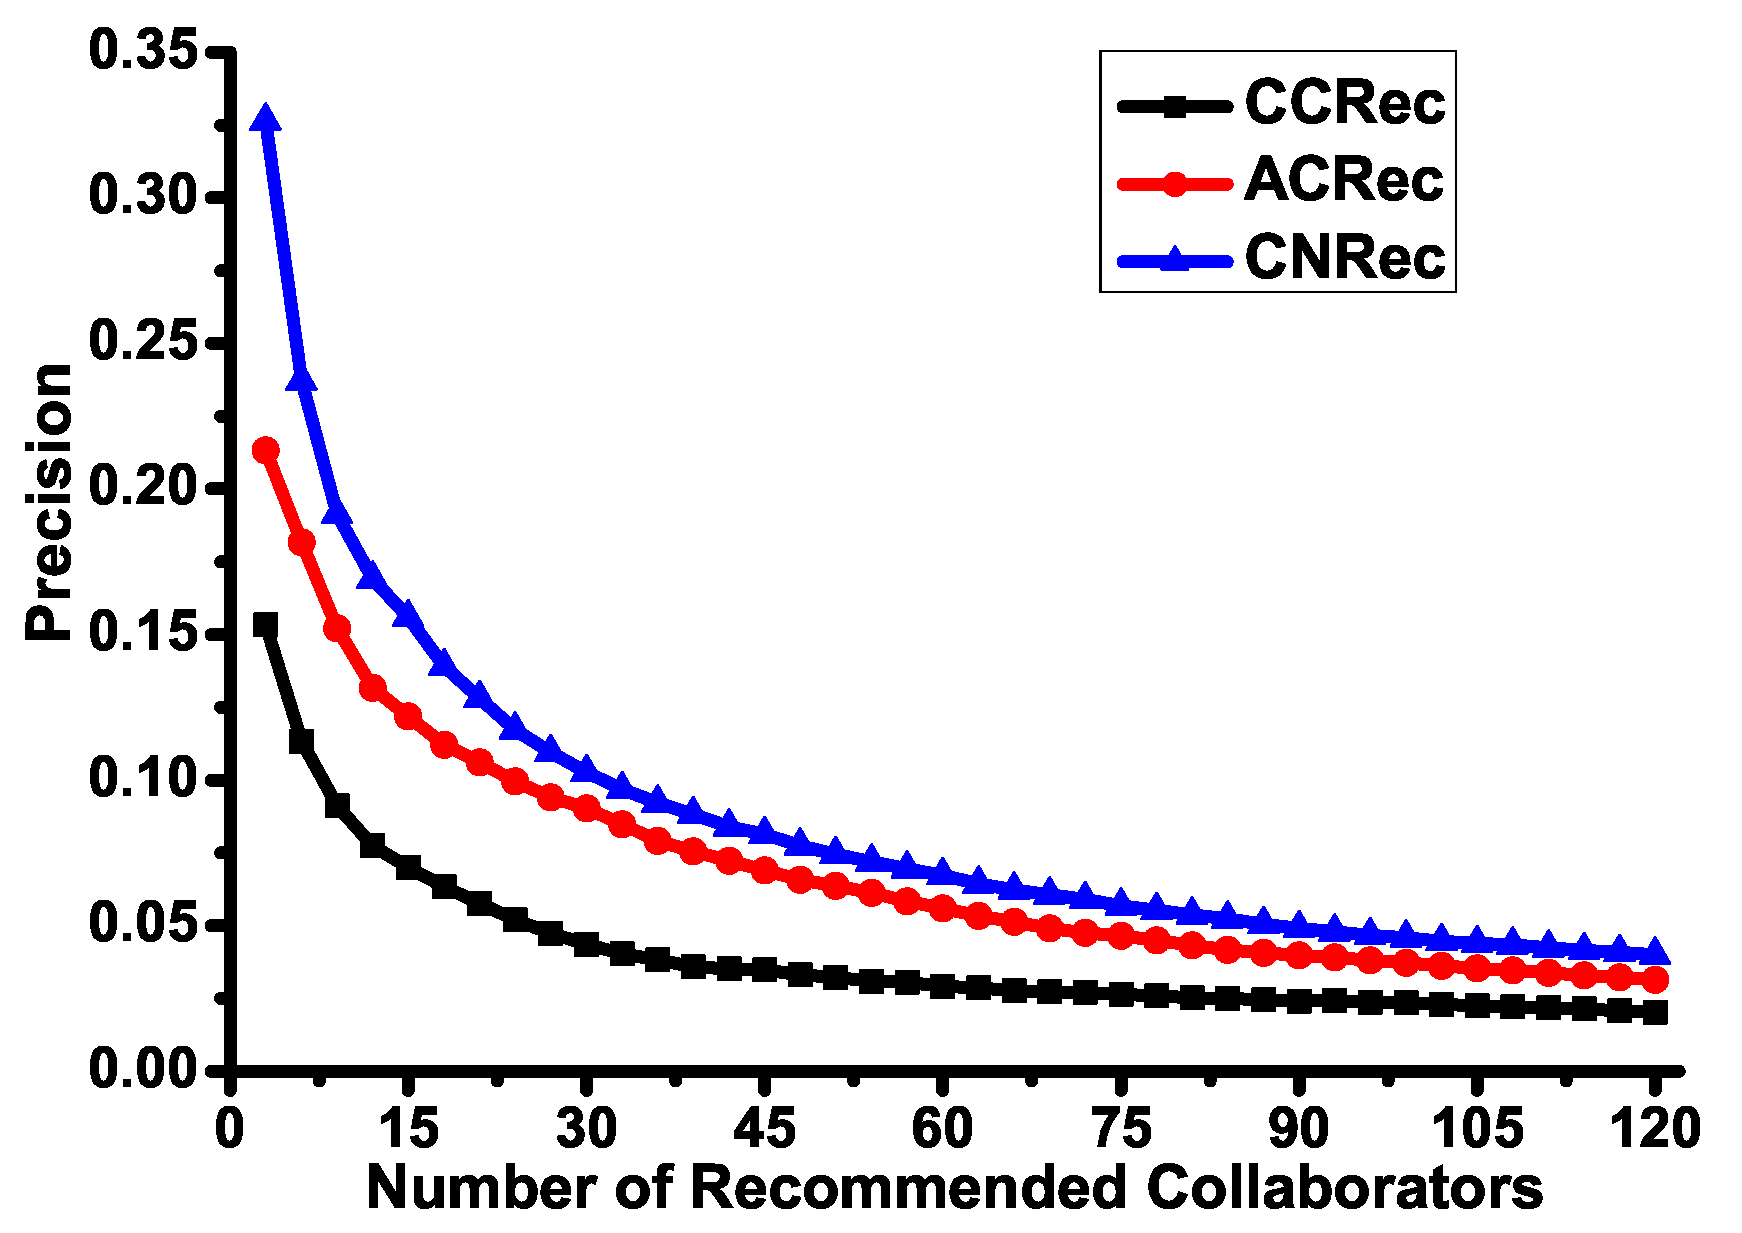
\includegraphics[width=0.31\textwidth]{Fig2-a.eps}}
\subfigure[Recall]{
\label{fig:2-b}
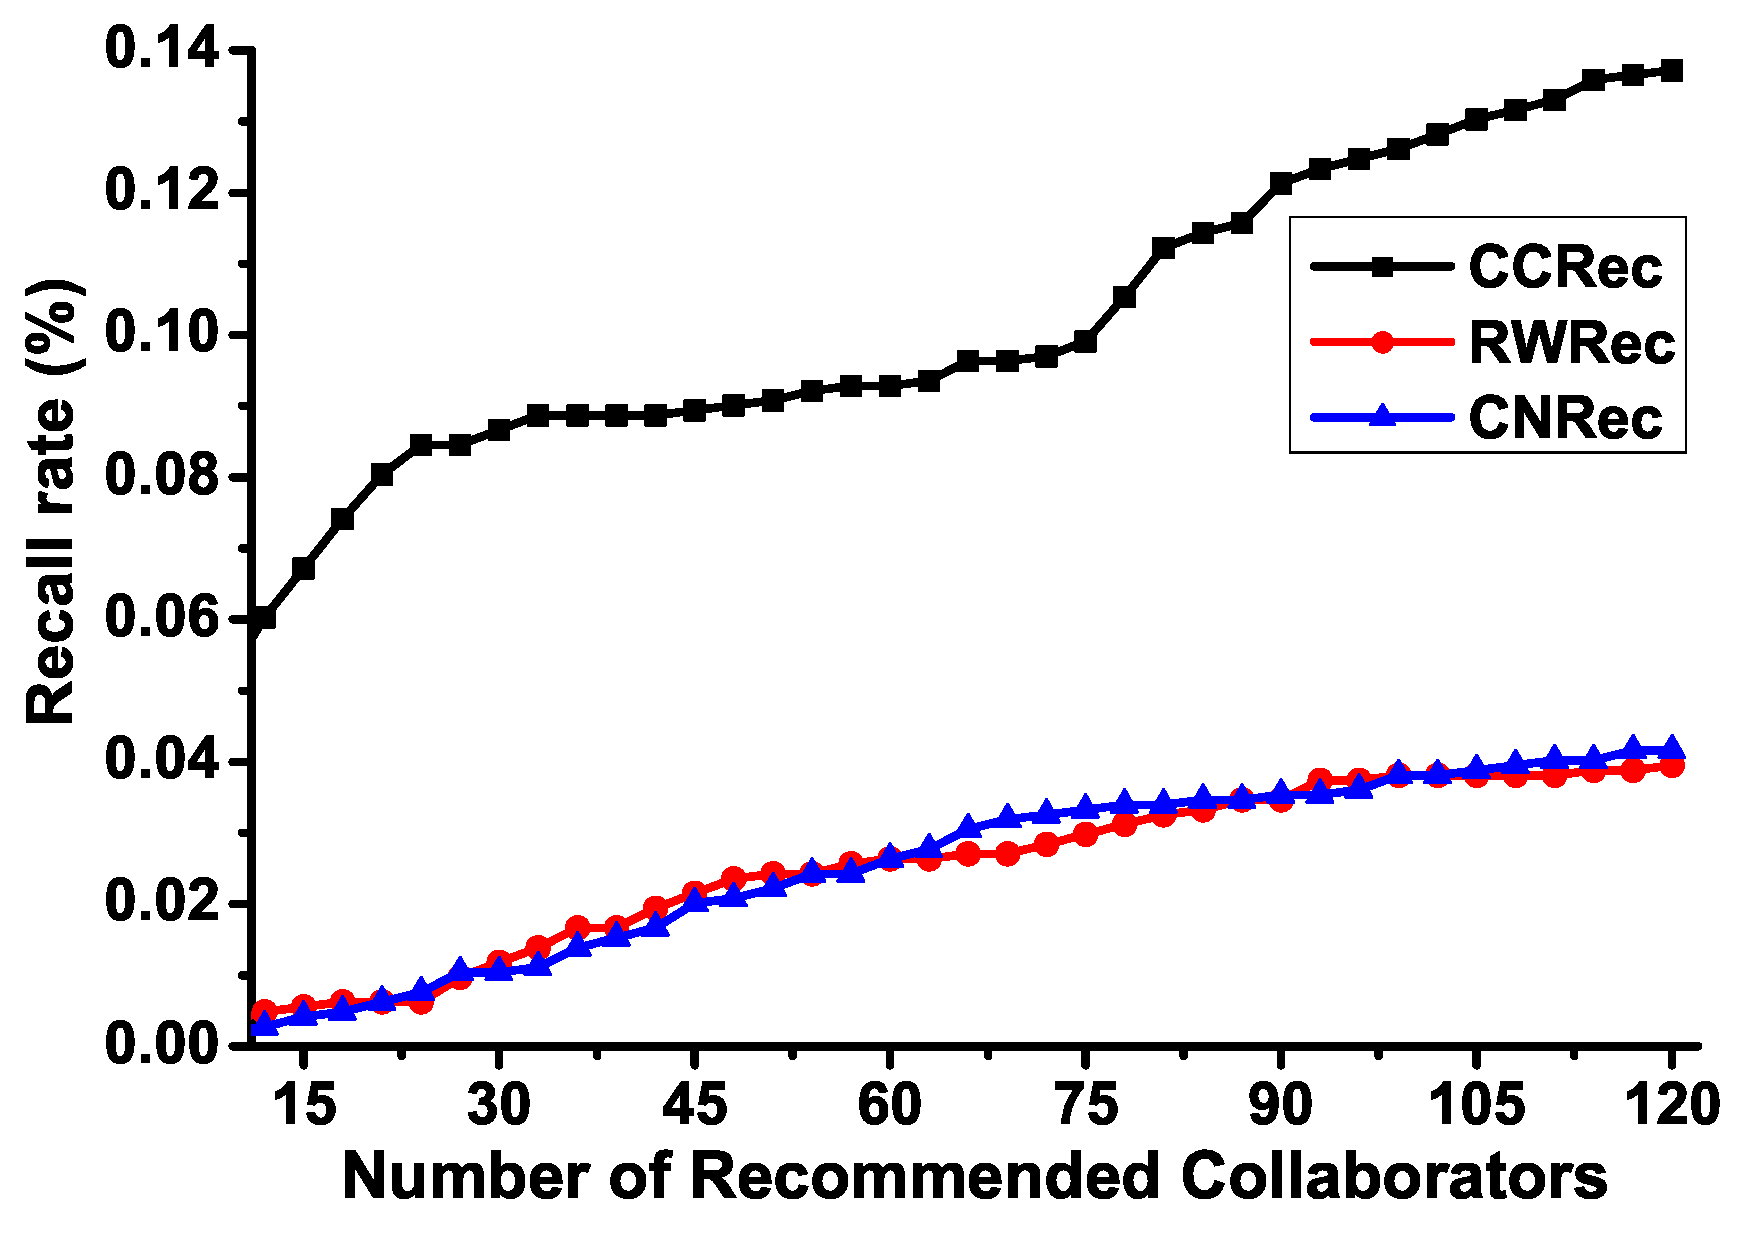
\includegraphics[width=0.31\textwidth]{Fig2-b.eps}}
\subfigure[F1]{
\label{fig:2-c}
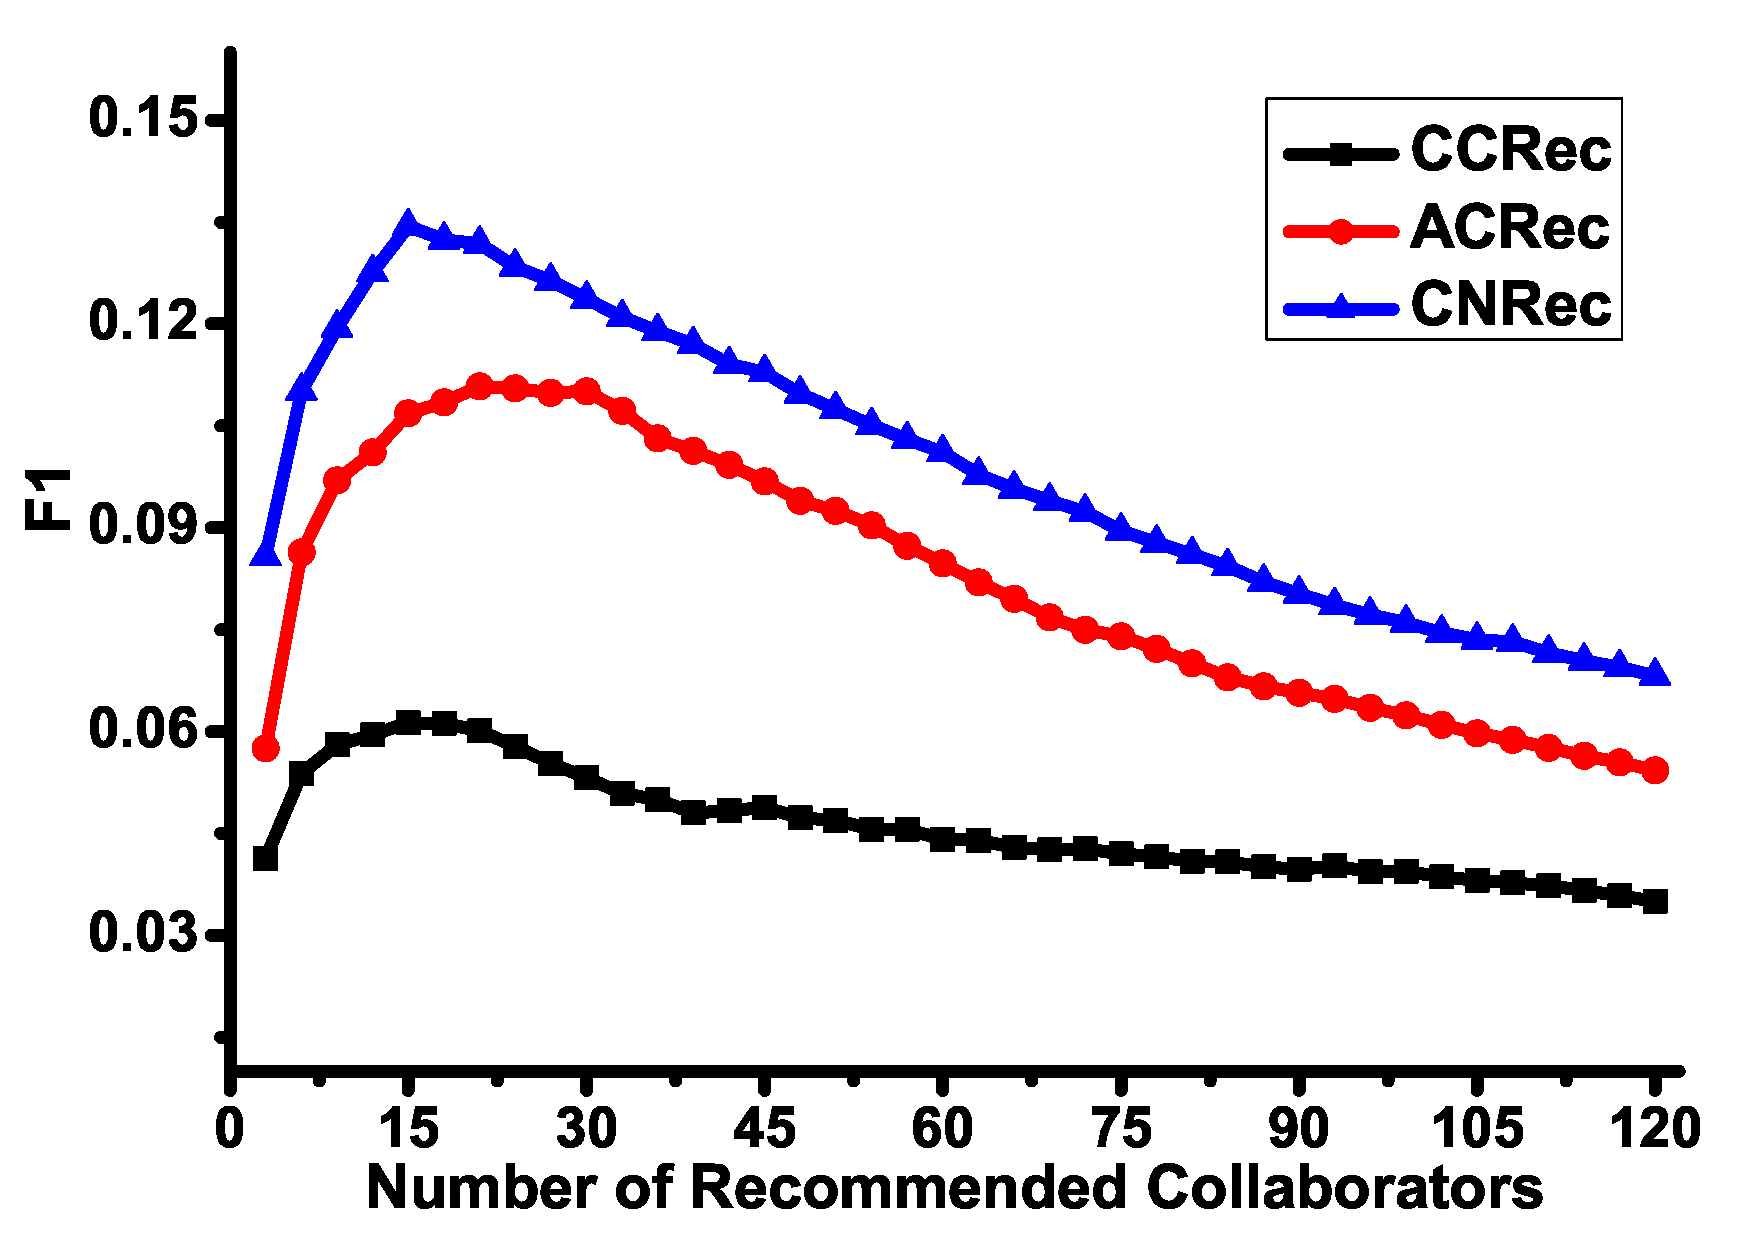
\includegraphics[width=0.31\textwidth]{Fig2-c.eps}}
\caption{Performance of CCRec and ACRec on most valuable collaborators recommendation}
\label{fig:2}
\end{figure*}

As shown in Fig. 3, The number of recommended collaborators has an obvious influence on the metrics with a clear trend. In the case of CCRec, as shown in Fig. 3(a), the precision drops when the number of recommended collaborators is increasing. At the same time, the recall in Fig. 3(b) rises with the increase of recommendation list, which finally approximates to $20\%$. In the case of ACRec, it has the same trend with CCRec in terms of precision and recall. Thus it can be verified that precision and recall are a pair of contradictory metrics. In order to weigh the two metrics to maximize profit, G. Shani et al. \cite{shani2011evaluating} adopted the metric $F1$. Fig. 3(c) describes the performance of CCRec and ACRec on $F1$. In case of CCRec model, $F1$ generally increases until the number of recommended collaborators is over 15, and then decreases gradually. Since point 15 is exactly the peak of $F1$. We can see that, CCRec performs best when recommending 15 collaborators to each researcher, and the $F1$ can reach $6.13\%$. However, in this scenario, ACRec gets its' highest $F1$ score $11.01\%$ at point 30.

A reflection of Fig. 3 substantiates that ACRec outperforms CCRec in terms of generating the most valuable collaborators recommendation. This is because, ACRec is based on the link-importance guiding random walk, which considers the walk distance and rank score and seeks the most valuable collaborators who may have known each other before, or are active in adjacent circles. Thus, compared with ACRec, there is no obvious superiority for CCRec to find the most valuable collaborators in adjacent circles.

\subsection{Most Potential Collaborators Recommendation}
% -----------------------------------------------------------------------------
We define the Most Potential Collaborators as collaborators who are worthy of being recommended and have never cooperated with the target researcher. Generating recommendations pertaining to the most potential collaborators is of great significance as the new collaborators are more meaningful and practical in the reality of academia. In this section, we explored the performance of CCRec, ACRec and CCRec on making most valuable collaborators recommendation.

\begin{figure*}
\centering
\subfigure[Precision]{
\label{fig:3-a}
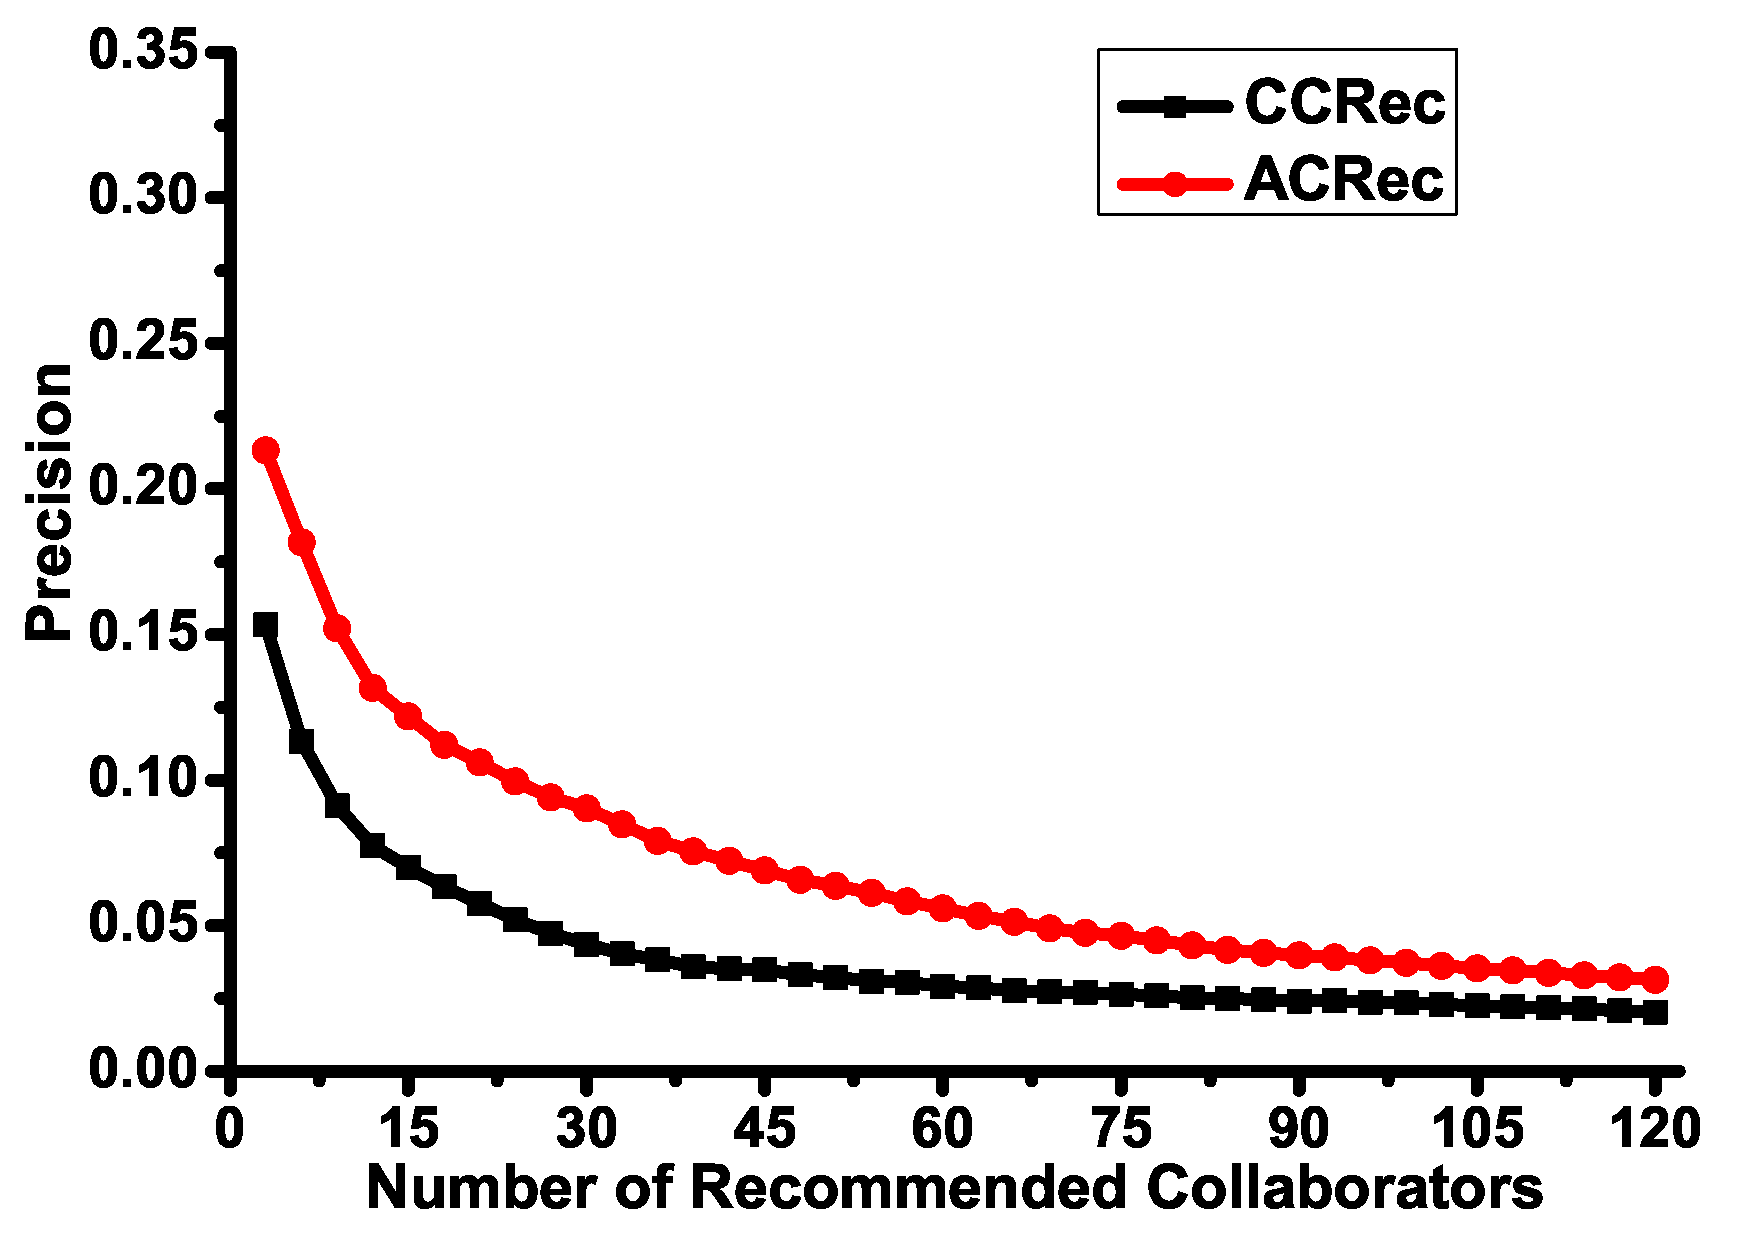
\includegraphics[width=0.31\textwidth]{Fig3-a.eps}}
\subfigure[Recall]{
\label{fig:3-b}
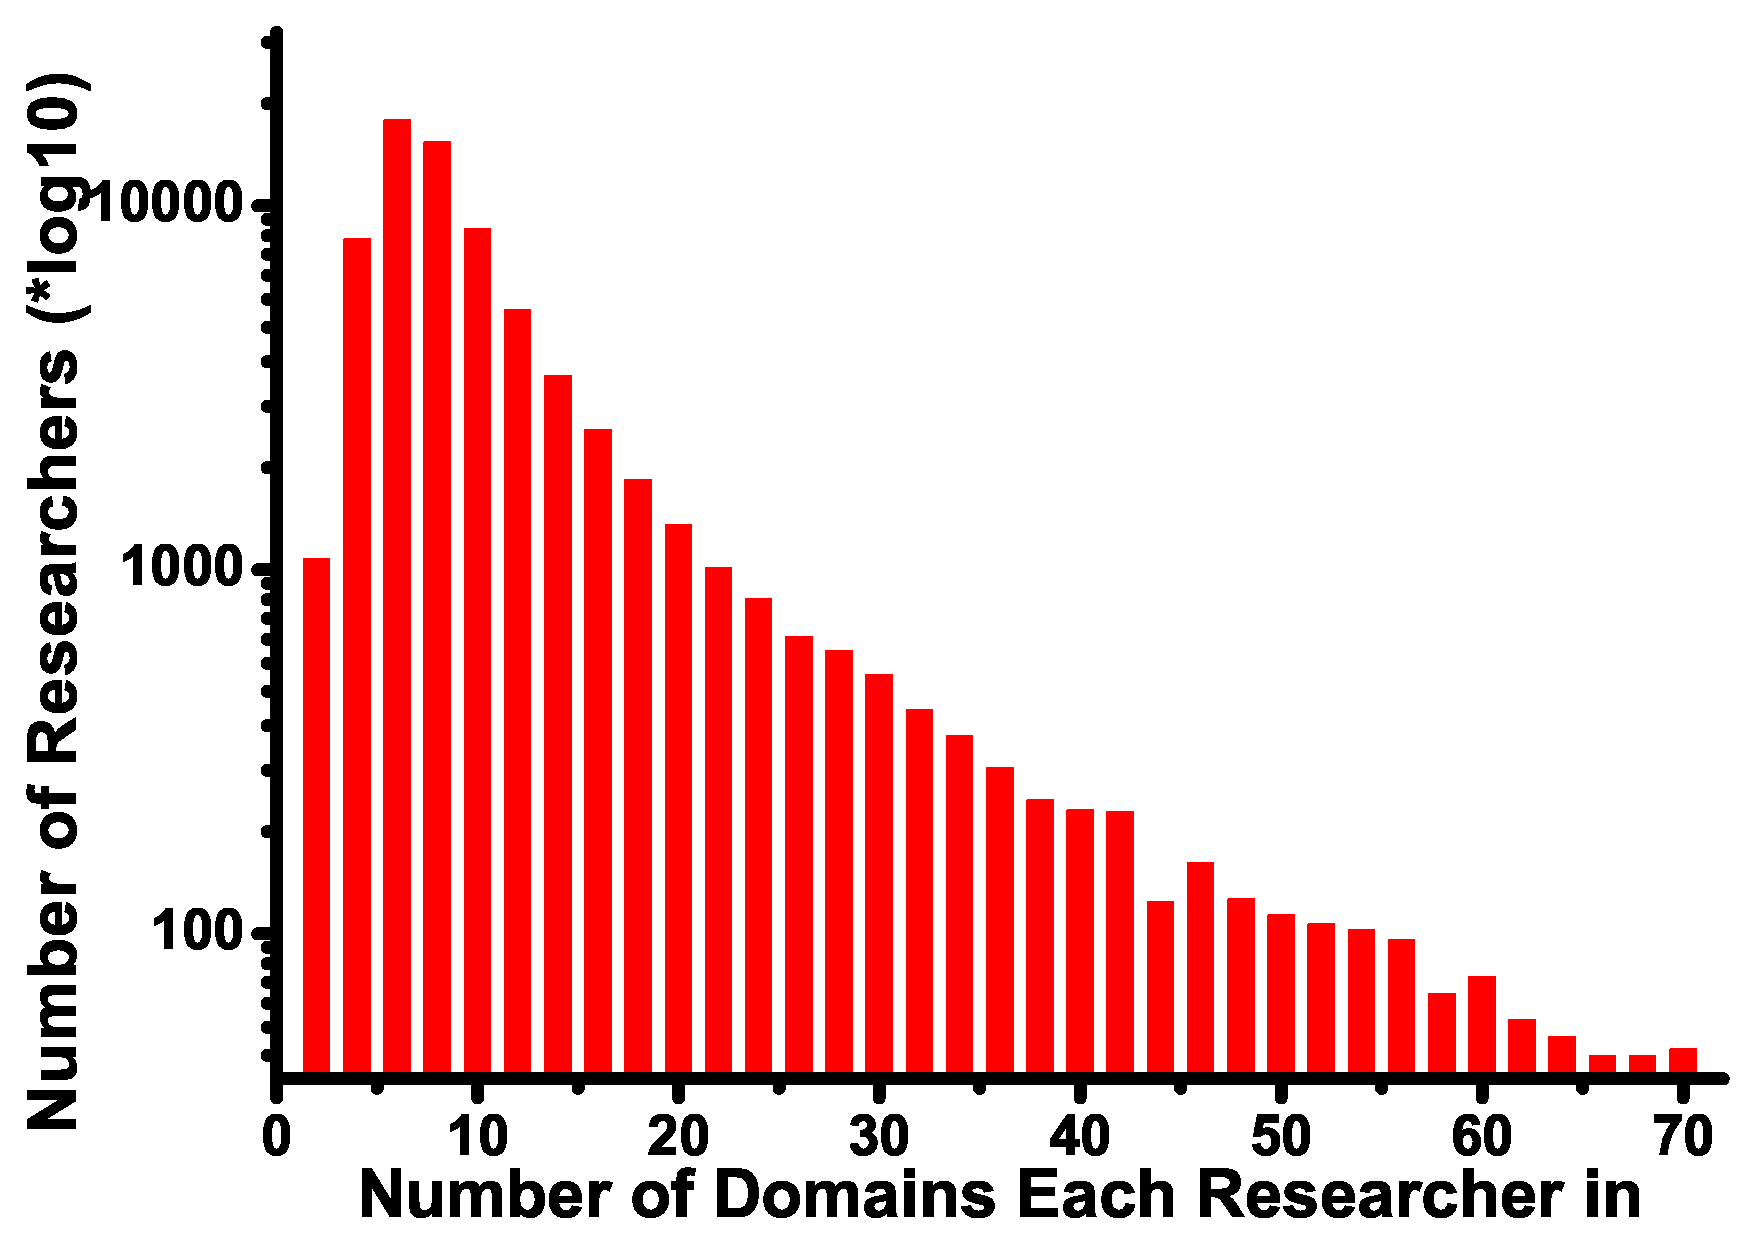
\includegraphics[width=0.31\textwidth]{Fig3-b.eps}}
\subfigure[F1]{
\label{fig:3-c}
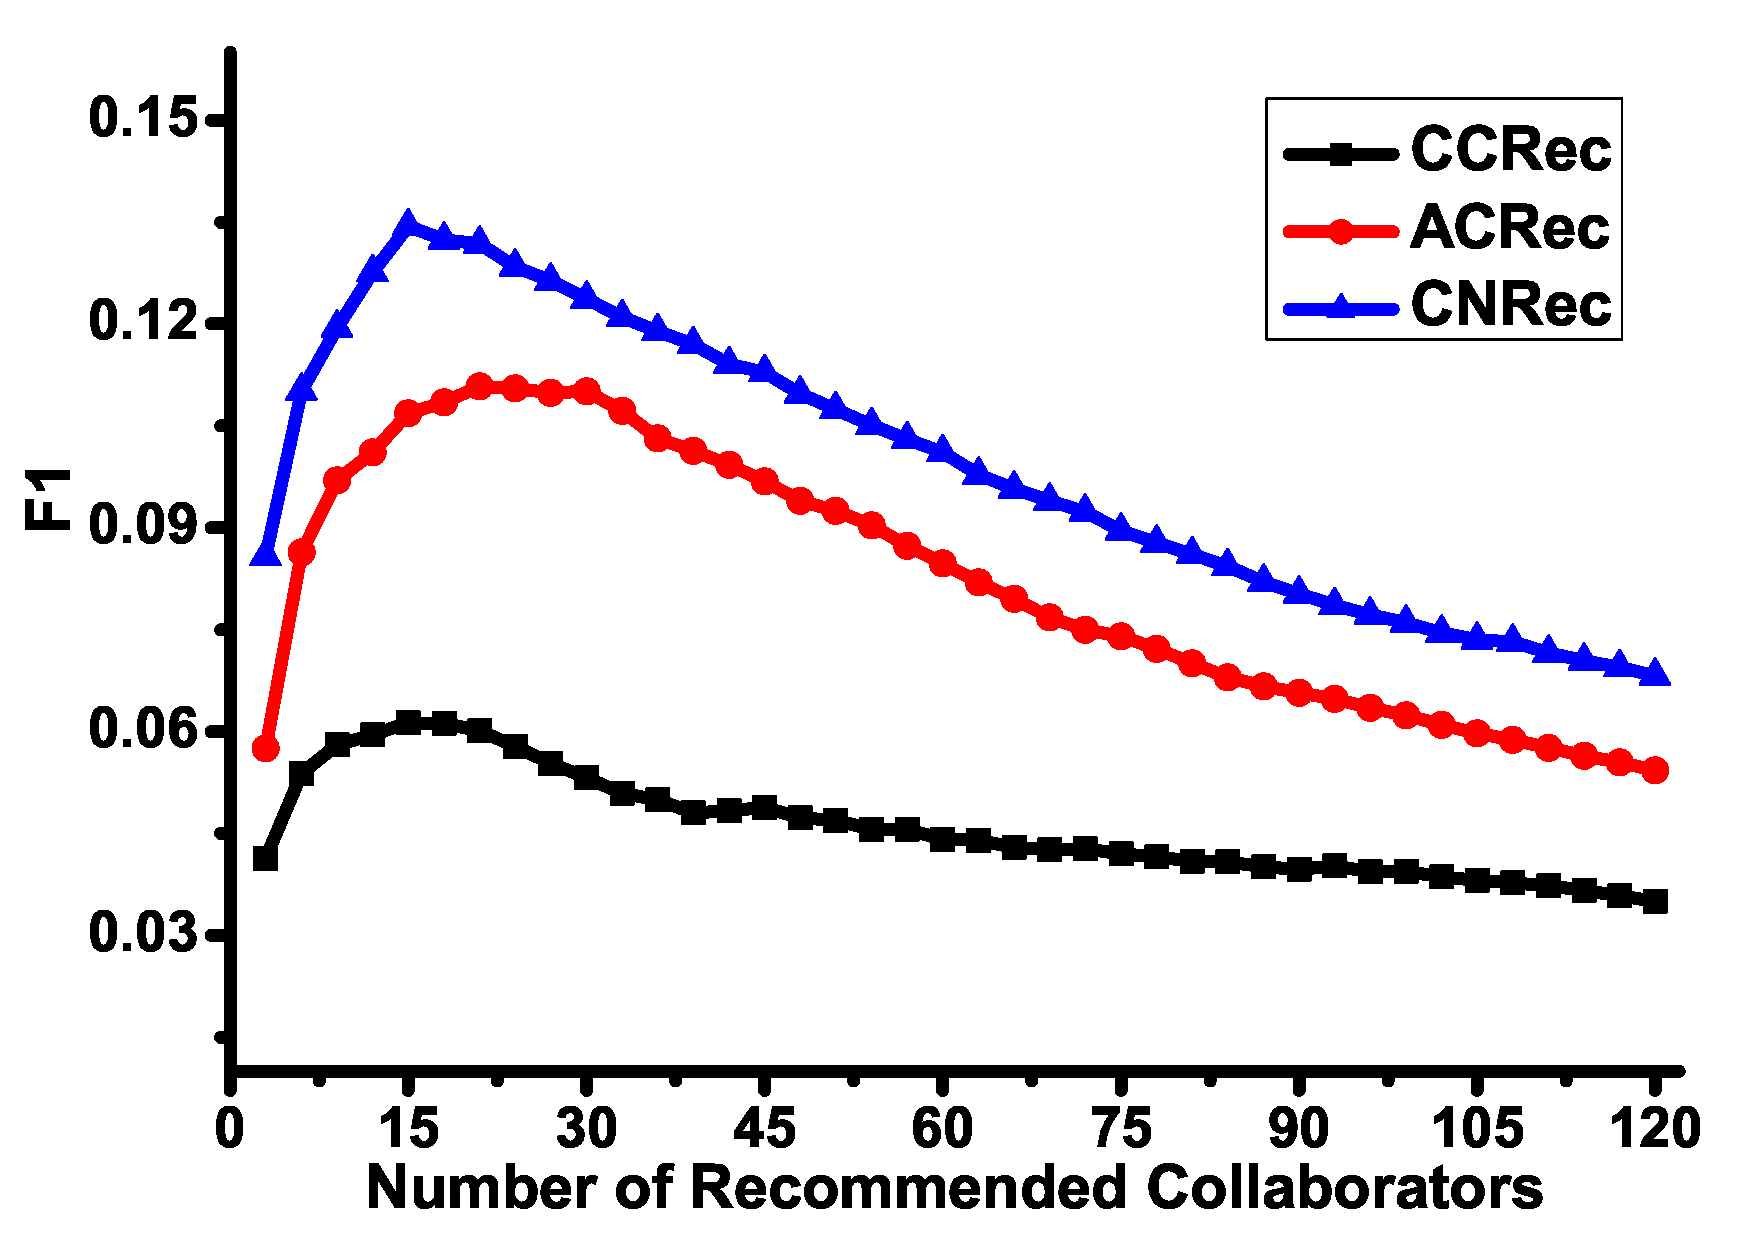
\includegraphics[width=0.31\textwidth]{Fig3-c.eps}}
\caption{Performance of CCRec, ACRec and CNRec on most potential collaborators recommendation}
\label{fig:3}       % Give a unique label
\end{figure*}

Figure 4 shows the performance of CCRec, ACRec and CNRec in terms of precision, recall and $F1$ with the number of recommended collaborators increasing. It can be observed that CCRec significantly outperforms ACRec and CNRec all the time on these three metrics. CCRec shows a downwards trend for precision and an upwards trend for recall rate. In the case of $F1$, it reaches a peak of $4.18\%$ when recommending 21 researchers. From Fig. 3, it is also evident that in relation to the generation of the most potential collaboration recommendations, ACRec outperforms CCRec in terms of the evaluation metrics we utilized.

In a nutshell, CCRec outperforms ACRec and CNRec with higher precision, recall and $F1$ on making the most potential collaborators. We analysed the theory. Each researcher is represented by the feature vector, as well as CCRec model which combines publications contents and collaboration networks to define the vector. Such a procedure has distinct advantages (e.g. rich information, more accurately to represent researchers' feature) in recommending new collaborators.

\subsection{Impact of clustered Domains number}
% -----------------------------------------------------------------------------
In this section, we exploit the impact of clustered domains number on the performance of CCRec. We adopted the following experiment settings: (1) Evaluate how the $F1$ changes with the number of collaborators recommended, (2) Generate the most potential collaborators recommendation for those 100 researchers selected above and (3) Recommend 21 potential collaborators for each researcher. Fig. 5 shows the experimental results.

\begin{figure*}
\centering
\subfigure[Precision]{
\label{fig:6-a}
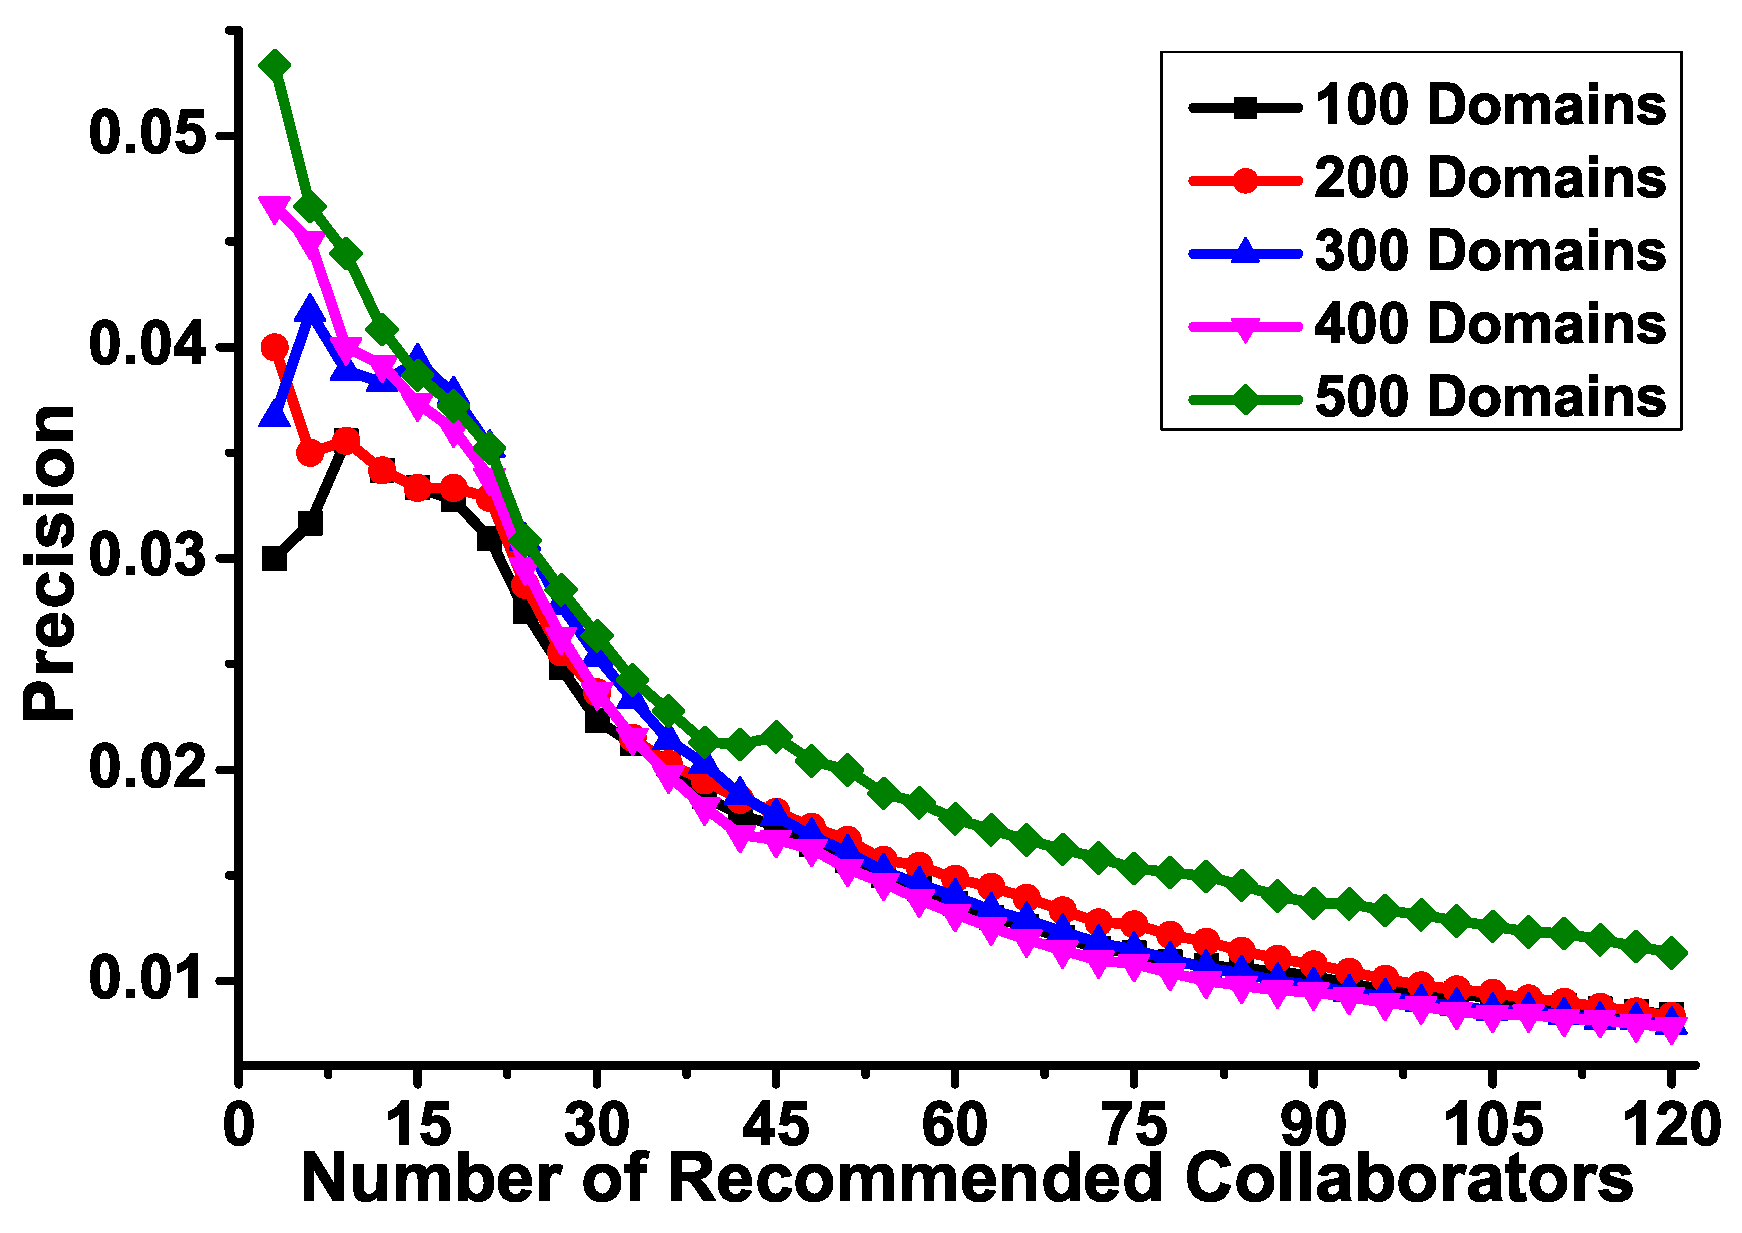
\includegraphics[width=0.31\textwidth]{Fig6-a.eps}}
\subfigure[Recall]{
\label{fig:6-b}
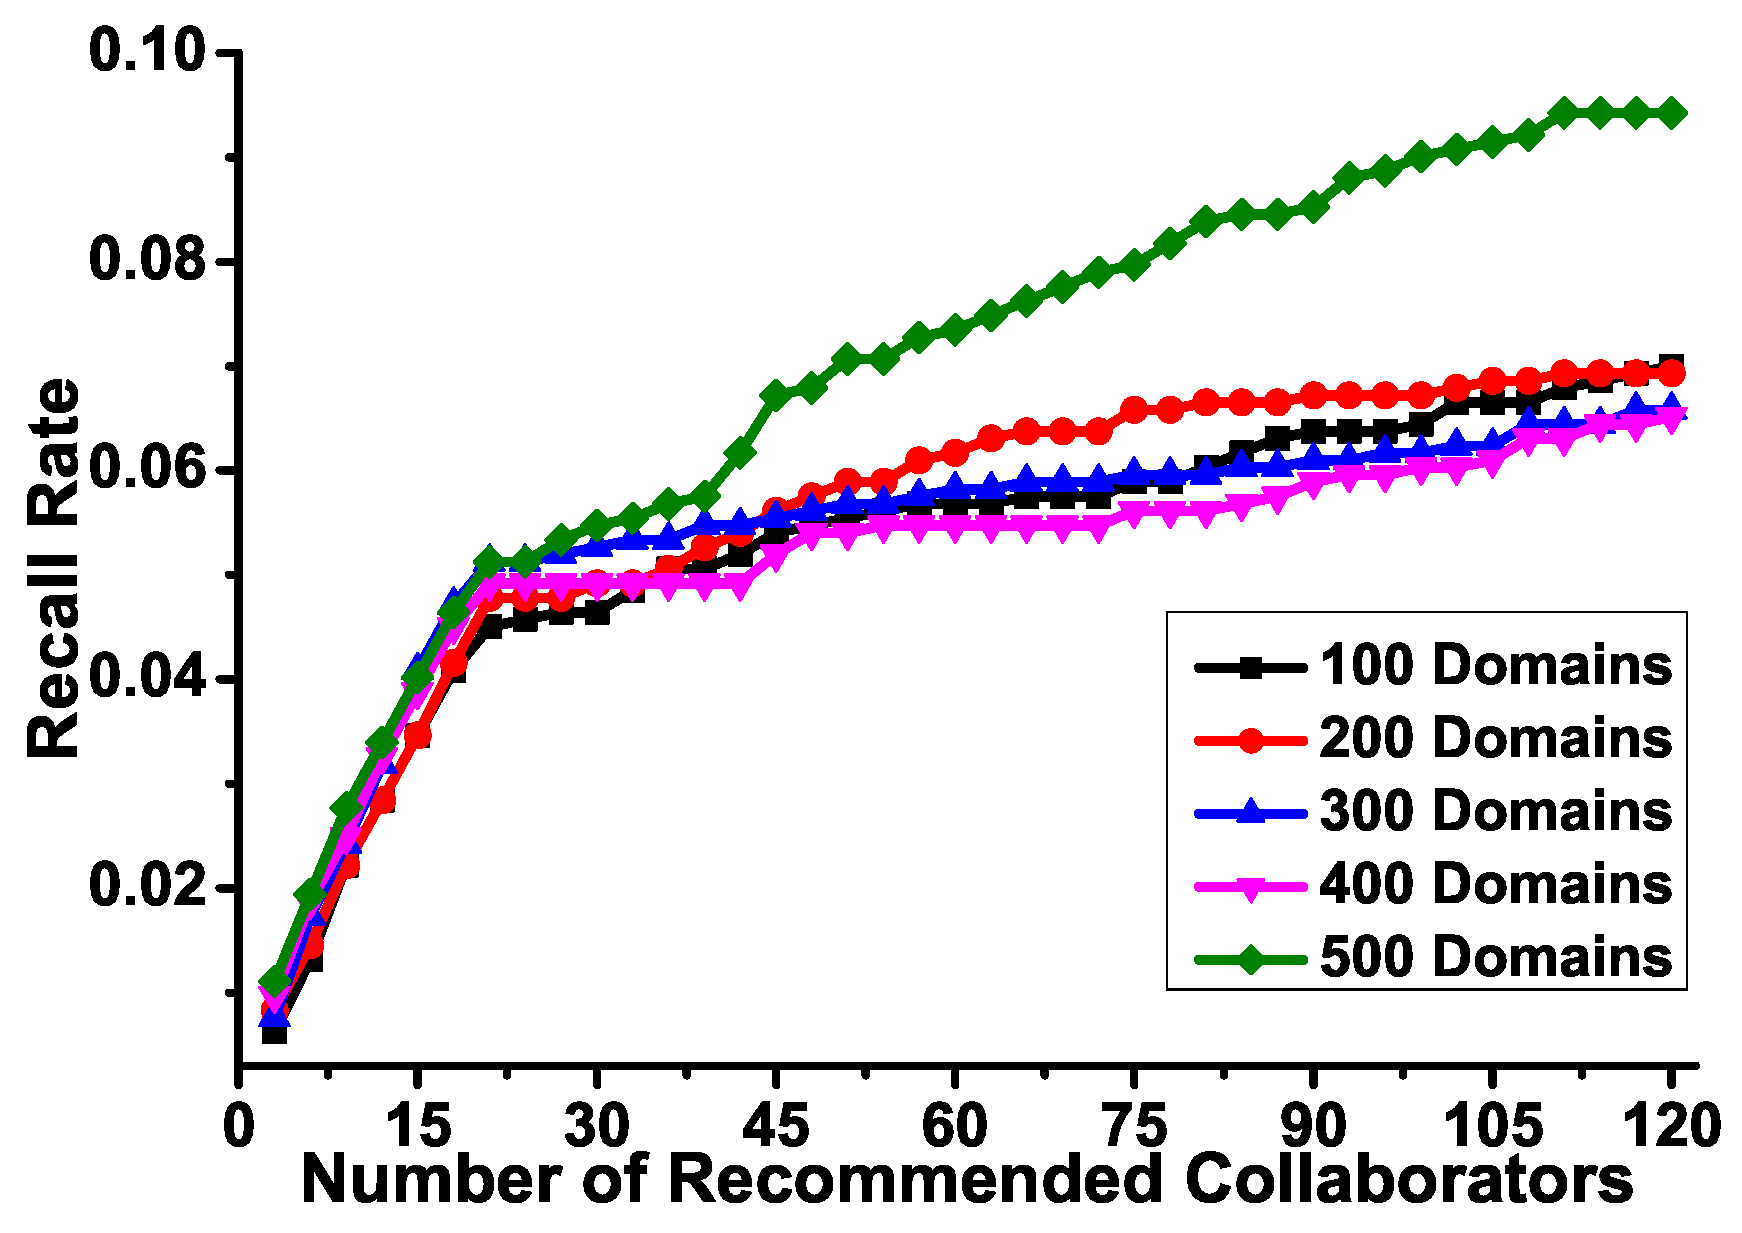
\includegraphics[width=0.31\textwidth]{Fig6-b.eps}}
\subfigure[F1]{
\label{fig:6-c}
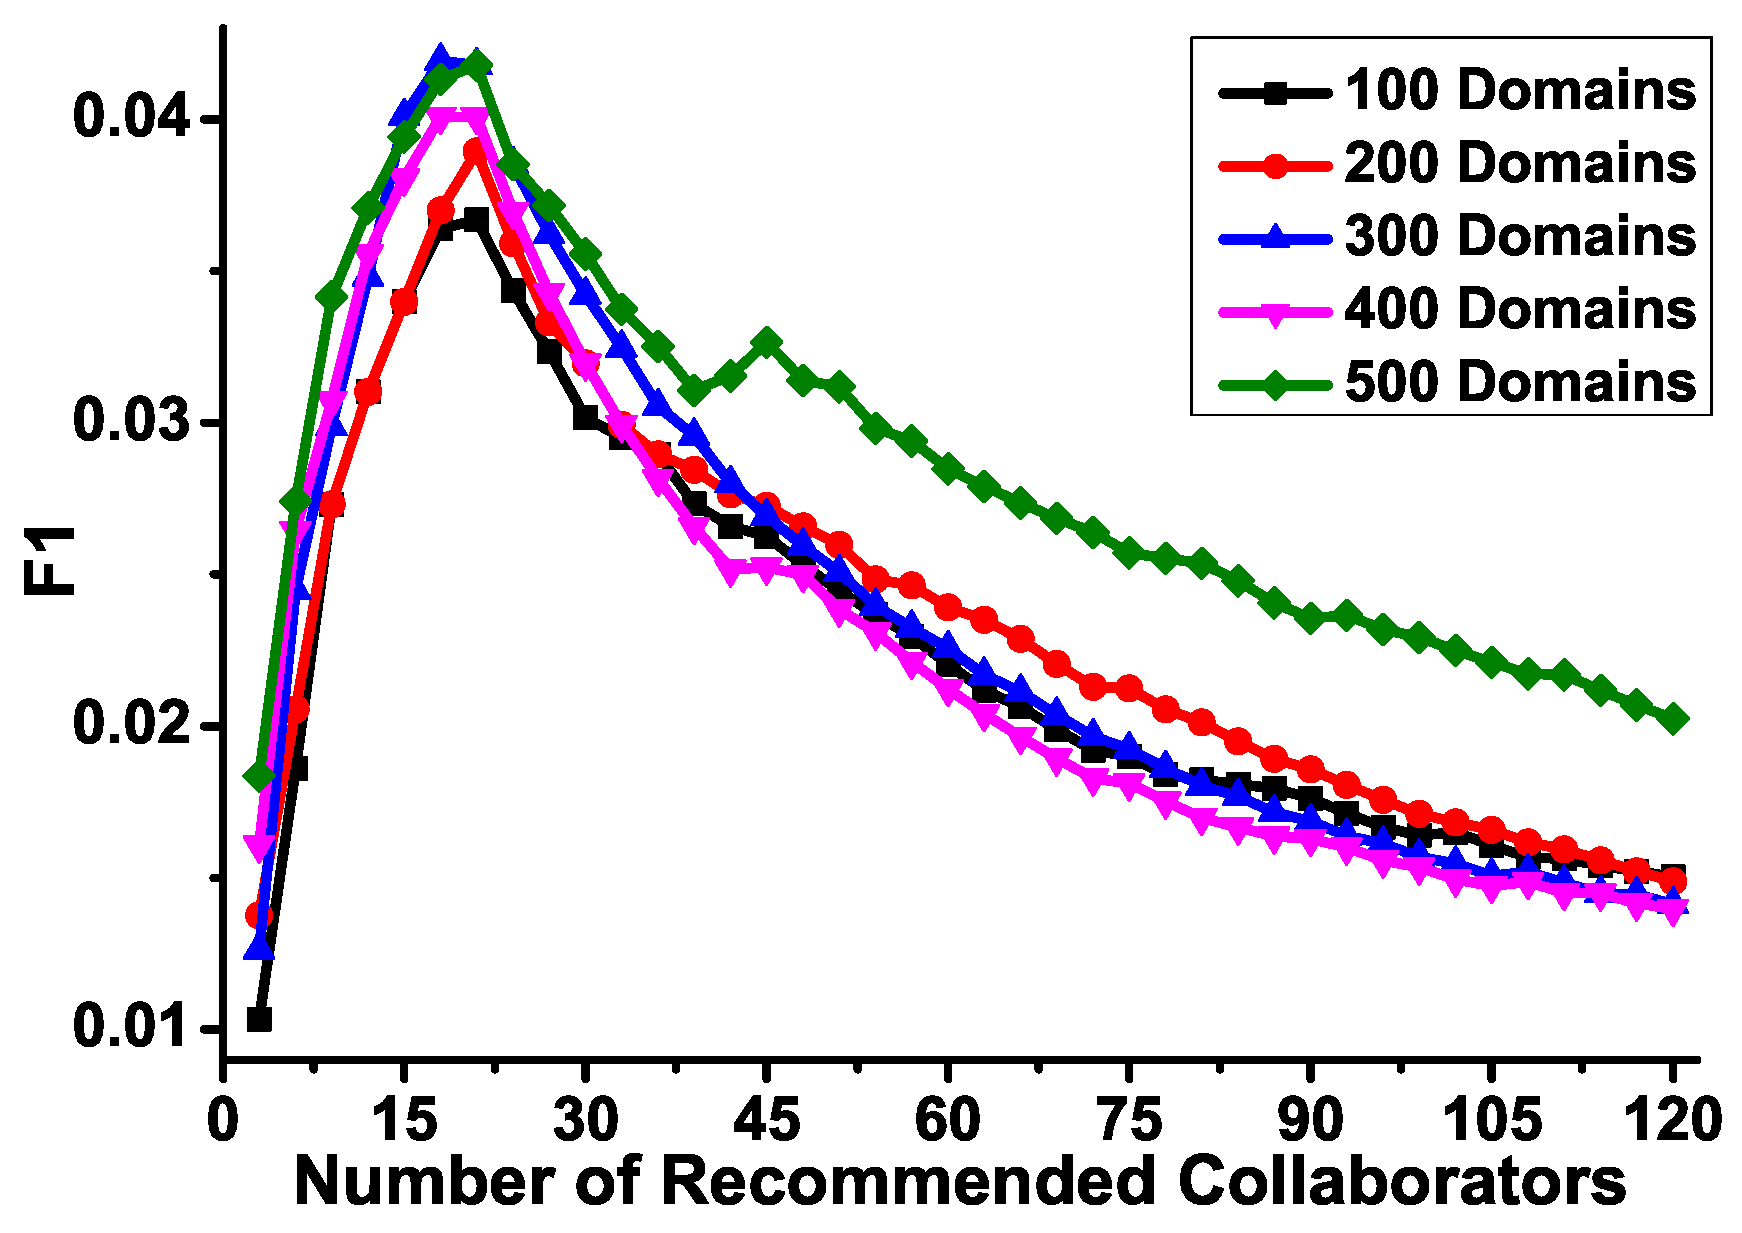
\includegraphics[width=0.31\textwidth]{Fig6-c.eps}}
\caption{The impact of clustered domains number on CCRec}
\label{fig:6}
\end{figure*}

\begin{figure}
\centering
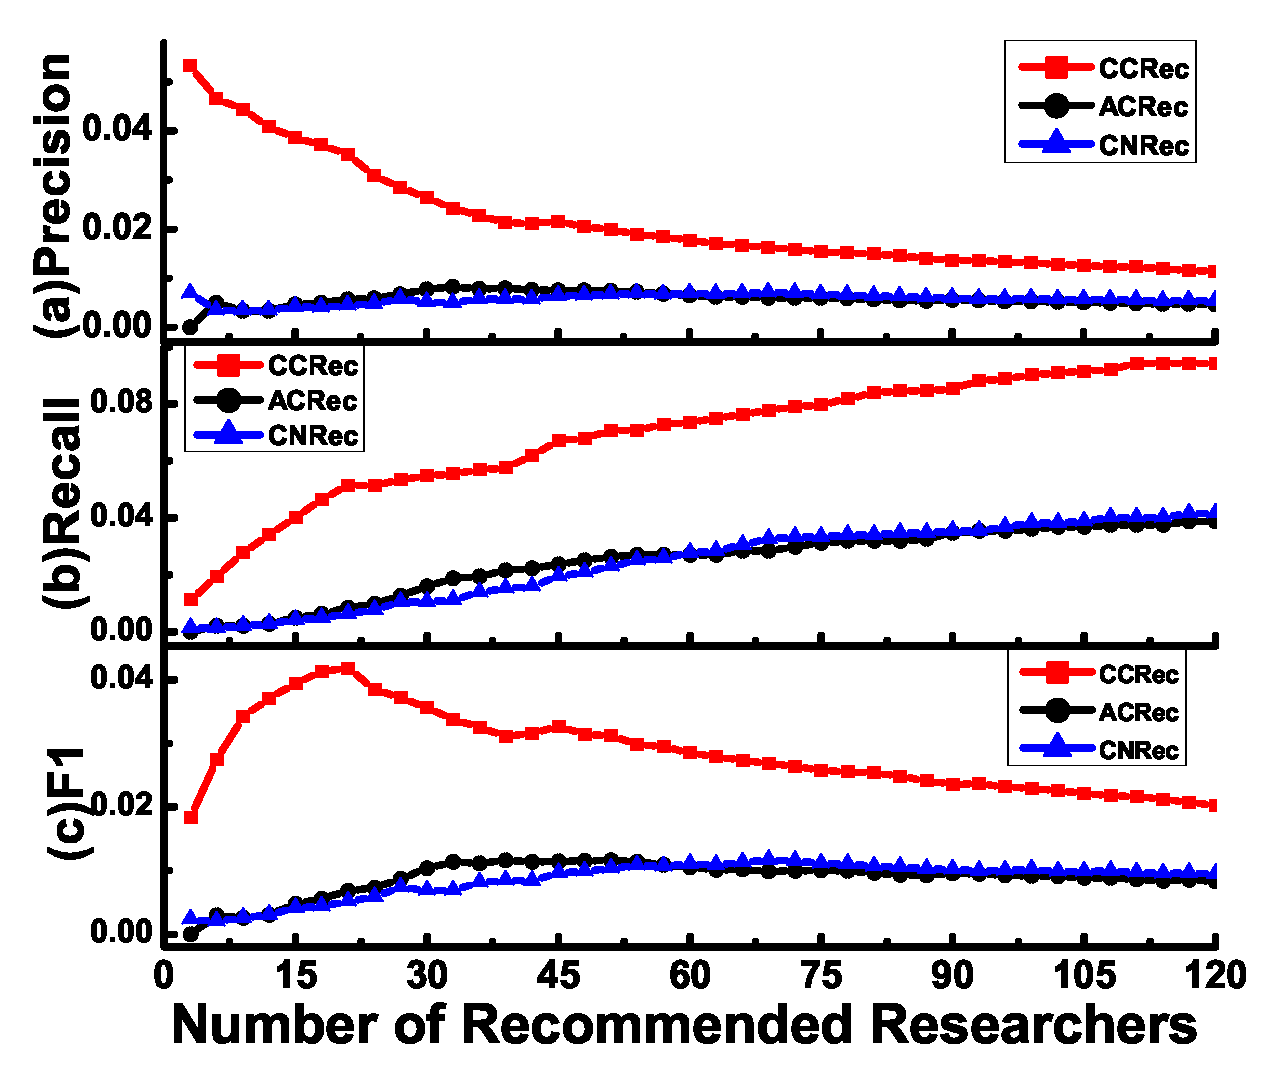
\includegraphics [width=3.4in]{Fig4.eps}
\caption{The impact of clustered domains number on CCRec}
\end{figure}

According to Fig. 5, the number of clustered domains does have certain effects on the performance of CCRec. If the number of clustered domains is appropriate, the $F1$ score achieves some enhancement. In this situation, when clustering the data mining academia into 300 or 500 domains, CCRec performs best for $F1$, when it reaches $4.18\%$.

In summary, our proposed model, which combines content-based and social network-based methods is really effective. Furthermore, in terms of precision, recall and $F1$, CCRec outperforms ACRec and CNRec generating the most potential collaborators (MPCs) recommendations for academic researchers.
% =============================================================================
\section{Conclusions}
% =============================================================================
In this paper, we focused on how to find researchers' MPCs based on big scholarly data which is necessary in current academia. To this end, we proposed a novel recommendation model called CCRec, by combining the features of publications content and collaboration networks. A topic clustering model and a random walk model were adopted to obtain scholars features, and make MPCs recommendation for researchers. We conducted extensive experiments on a subset of DBLP data set to evaluate the performance of CCRec in comaprison to other state-of-the-art methods, namely: ACRec and CNRec. Our experimental results show that, CCRec outperforms ACRec and CNRec in terms of precision, recall and $F1$ score. Due the the utilization of a topic clustering model, the problem of topic drift in academic research has been solved to some extent.

Our research on CCRec reveals that the combination of content-based and network-based methods can improve the generation of effective academic collaborations. Nonetheless, there is still room for future study in this direction. We extracted the titles of publications as the corpus of the topic clustering model, which are not more comprehensive than the abstract and main body of publications. Additionally, specific evaluation metrics should be utilized to evaluate the topic drift problem. As the future work, more experiments and studies should be conducted.

\section*{References}

\bibliography{CCRec-Full}

\end{document}
